% Latex Beamer template following CERN template guidelines (or trying!)

\documentclass[aspectratio=169]{beamer}
\usepackage{xcolor}
\usepackage{graphicx}
\usepackage{multicol}
\usepackage{tikz}

% Code listings with syntax highlighting
%  Require Pygments
\usepackage{minted}

\usetheme{CERN}

\newcommand{\interludeTitle}{We are here!}
\AtBeginSection[] {
    \frame{
	\frametitle{\interludeTitle}
      \begin{multicols}{2}
        \tableofcontents[
            currentsection,
            sectionstyle=show/shaded,
            ]
	  \end{multicols}
    }
}

\AtBeginSubsection[] {
	  \frame{
		\frametitle{\interludeTitle}
		\begin{multicols}{2}
        \tableofcontents[
            currentsubsection,
            subsectionstyle=show/shaded,
            ]
		\end{multicols}
	  }
}


% Talk date
% Uncomment this to define a presentation date distinct from \today
% \def\mydate{20 Feb 2000}

% Preamble
\title[]{Title}
\subtitle{Subtitle}
\author[Author]{\texorpdfstring{\url{name.surname@cern.ch}}{Author}}

% Body
\begin{document}
    
    \cernSplashBlue

    % Title
    {
    \setbeamertemplate{footline}{}
    \setbeamertemplate{navigation symbols}{}
    \frame{\titlepage}
    }
    \setcounter{framenumber}{0}

    % TOC
    \frame{
        \frametitle{Table of Contents}
        \begin{multicols}{2}
            \tableofcontents
        \end{multicols}
    }



    \section{Introduction}
    
    \frame{
        \frametitle{This is the first slide}
        %Content goes here
        \begin{block}{Ideas}
            See how this loooks
        \end{block}
        \begin{itemize}
            \item Item 1
            \item Item 2
        \end{itemize}
    }

	% This block includes a picture full slide
	{ % all template changes are local to this group.
		\setbeamertemplate{navigation symbols}{}
		\begin{frame}[plain]
			\begin{tikzpicture}[remember picture,overlay]
			\node[at=(current page.center)] {
				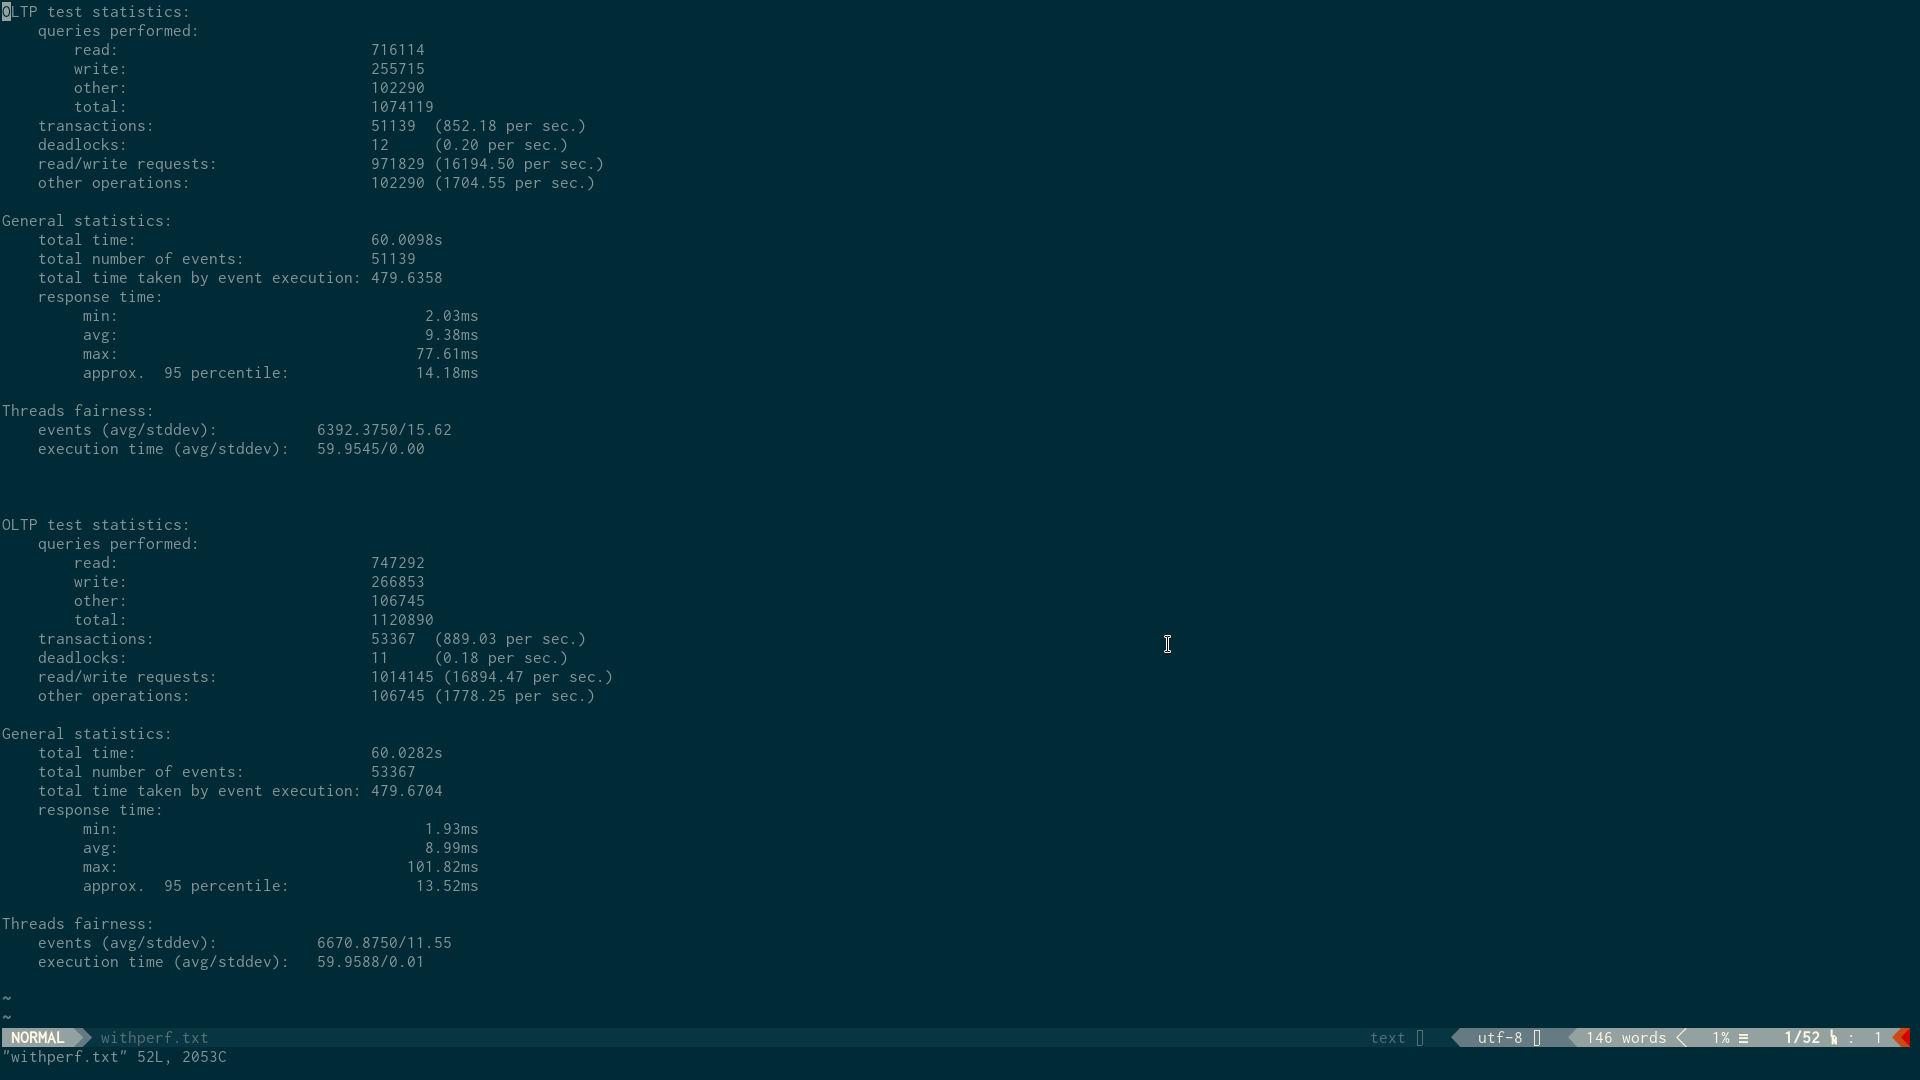
\includegraphics[width=\paperwidth]{images/image.png}
			};
			\end{tikzpicture}
		\end{frame}
	}

    % This slide has code block with syntax highlighting using the Minted package
    %  Minted requires Pygments and building the PDF with the --shell-escape argument
    %  for pdflatex
    \begin{frame}[fragile]
        \frametitle{This slide has code blocks}
		\begin{minted}[
			frame=lines,
			framesep=2mm,
			baselinestretch=1.2,
			fontsize=\footnotesize,
			linenos
			]{python}
        import numpy as np
         
        def incmatrix(genl1,genl2):
            m = len(genl1)
            n = len(genl2)
            M = None #to become the incidence matrix
            VT = np.zeros((n*m,1), int)  #dummy variable
        \end{minted}
    \end{frame}


    \subsection{Intro subsection}
    \frame{
        \frametitle{This is the second slide}
        \framesubtitle{A bit more information about this}
        %More content goes here
        \begin{alertblock}{Alert block}
            Alert text
        \end{alertblock}
    }
    
    \section{Section 1}

    \frame{
        \frametitle{slide w/ pic included from local project folder}
        \framesubtitle{rather than generic include folder}

        \begin{tikzpicture}
        \node[at=(current page.center)] {
          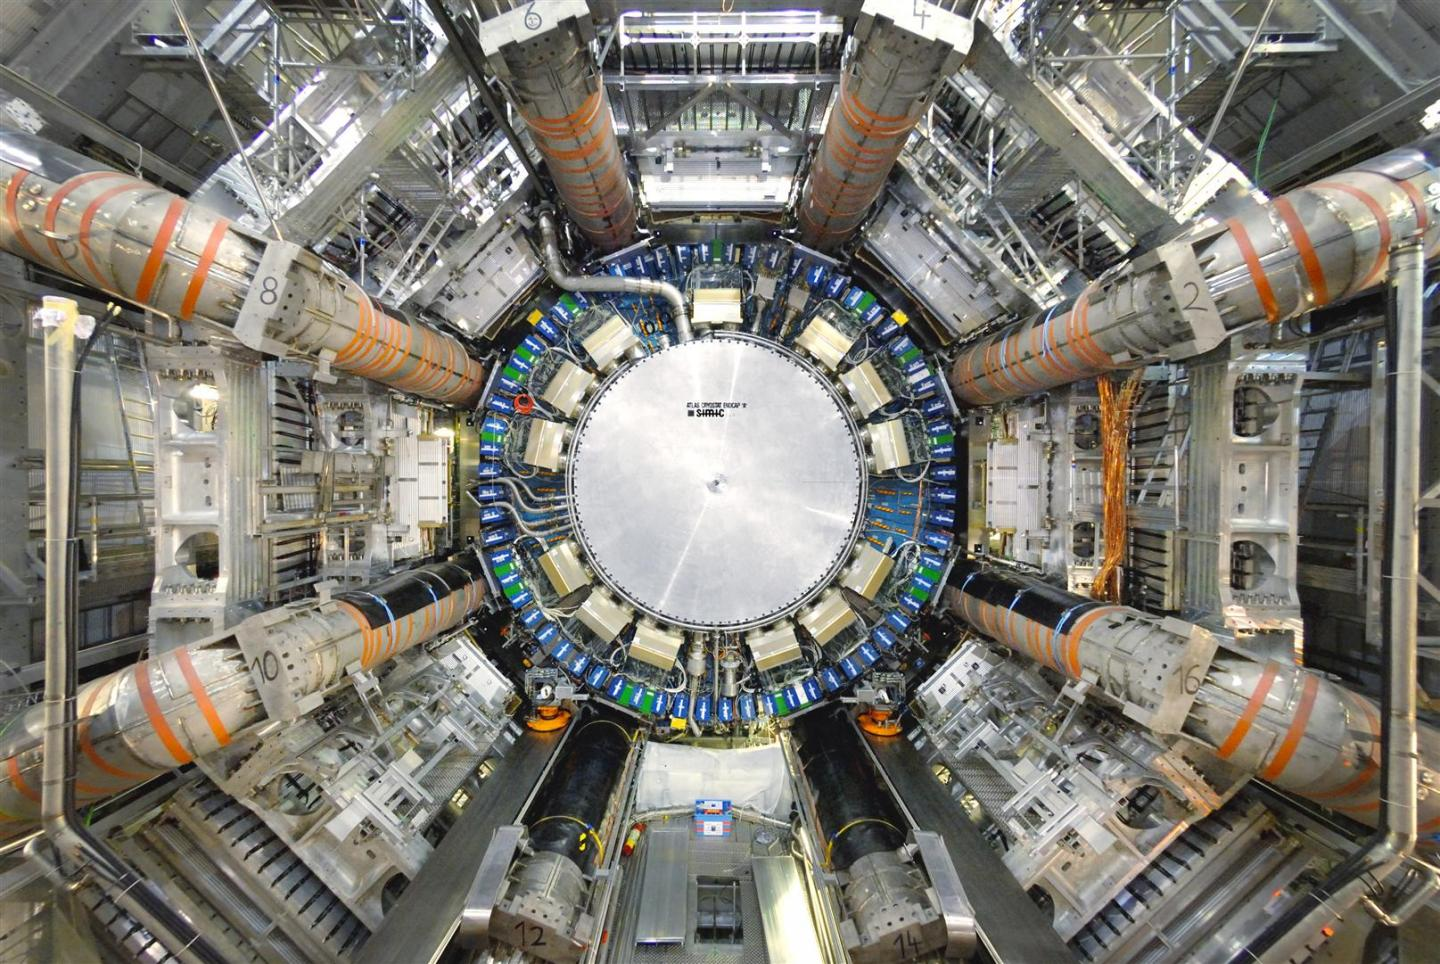
\includegraphics[width=0.55\paperwidth]{ex-figs/atlas.jpeg}
        };
        \end{tikzpicture}
        %More content goes here
    }
    \section{Section 2}

    \frame{
        \frametitle{Generic slide}
        \framesubtitle{A bit more information about this}
        %More content goes here
    }

    
    \section{Conclusion}
    
    \frame{
        \frametitle{Generic slide}
        \framesubtitle{A bit more information about this}
        %More content goes here
    }
    
    \section{Acknowledgements}
    
    \frame{
        \frametitle{Generic slide}
        \framesubtitle{A bit more information about this}
        %More content goes here
    }

    \section{}
    \cernSplashWhite

\end{document}

